\documentclass[usenames,dvipsnames,11pt]{beamer} 

\usepackage[utf8]{inputenc}
\usepackage{verbatim}
\usetheme{umu}

%%% Bibliography
\usepackage[style=authoryear,backend=biber]{biblatex}
\addbibresource{bibliography.bib}

% Author names in publication list are consistent 
% i.e. name1 surname1, name2 surname2
% See https://tex.stackexchange.com/questions/106914/biblatex-does-not-reverse-the-first-and-last-names-of-the-second-author
\DeclareNameAlias{author}{given-family}

%%% Suppress biblatex annoying warning
\usepackage{silence}

%%% Some useful commands
% pdf-friendly newline in links
\newcommand{\pdfnewline}{\texorpdfstring{\newline}{ }} 
% Fill the vertical space in a slide (to put text at the bottom)
\newcommand{\framefill}{\vskip0pt plus 1filll}

%%% Enter additional packages below (or above, I can't stop you)! / Jesper
\renewcommand{\proofname}{\sffamily{Proof}}


\title[БГТУ им. В.Г.Шухова]{Разработка и реализация алгоритма вычисления уровня топлива в баках сложной конфигурации}
	\date[\today]{\small\today}
	\author[Иван Притчин]{
		Автор работы:\\
		Притчин Иван Сергеевич, магистрант МИВТ-191 \\
		\vspace{0.3cm}
		Руководитель:\\
		Зуев Сергей Валентинович, канд. ф-м наук\\	
	}
	

	
\institute{Кафедра программного обеспечения ВТ и АС}

\usepackage{ragged2e} % выравнивание
\usepackage{cancel}
\usepackage{lipsum}
\usepackage{hyperref}
\newcommand\Fontvi{\fontsize{7.5}{8.7}\selectfont}

\newtheorem{rtask}{Задача}
\newtheorem{rsolution}{Решение}

% анимация
\usepackage{xmpmulti}

\usepackage{xcolor,colortbl}

\usepackage{import}

\begin{document}

\begin{frame}
  \titlepage
\end{frame}

\begin{frame}{Актуальность}
	Компании, осуществляющие мониторинг за транспортными средствами, столкнулись с проблемой точности вычислений уровня топлива в баках сложной конфигурации:
	\begin{itemize}
		\item большое количество вариаций форм
		\item ограничения на стороне сервера у систем спутникового мониторинга в рассчете уровня топлива по данным, отсылаемых трекером;
		\item тяжелые условия эксплуатации, приводящие к колебаниям топлива.
	\end{itemize}
\end{frame}

\begin{frame}{Монтаж и тарировка ДУТ}
	\begin{minipage}[h]{0.39\linewidth}
		\begin{figure}
		\centering
		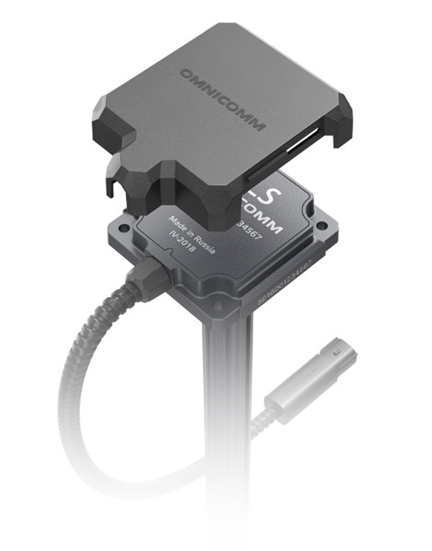
\includegraphics[width=1\linewidth]{graphics/screenshot002}
		\end{figure}
	\end{minipage}
	\hfill
	\begin{minipage}[h]{0.59\linewidth}
		\begin{itemize}
			\item Специалист сервисной службы осуществляет монтаж датчика уровня топлива (ДУТ) в бак
			\item Производится процесс тарирования. Повторяются следующие действия:
			\begin{itemize}
			\item Заливается $v_i$ литров в бак
			\item Снимаются показания $D_i$ с датчика
			\end{itemize}
		\end{itemize}
		В результате тарировки получаем функцию, заданную множеством точек:
		\{($D_i$, $V_i$)\},
		где $$V_i = \sum_{i}v_i$$
	\end{minipage}
\end{frame}

\begin{frame}{Процесс вычисления показаний с ДУТ}
	\begin{enumerate}
		\item Трекер считывает данные с датчиков и формирует сообщение
		\item Сообщение отправляется на сервер, на котором сохранена функция преобразования (тарировочная таблица):
		$$f:D \rightarrow V$$
		\item Если приходящее с трекера значение $D$ отсутствует в таблице, используются алгоритмы линейной интерполяции и экстраполяции для расчёта $V$
	\end{enumerate}
\end{frame}

\begin{frame}{Процесс вычисления показаний с ДУТ}
	\begin{minipage}[h]{0.39\linewidth}
			\begin{figure}
			\centering
			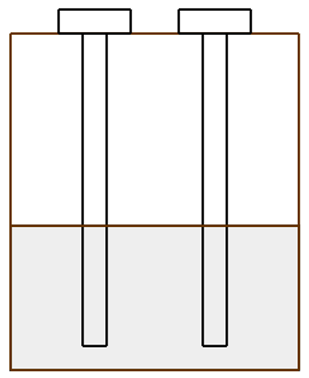
\includegraphics[width=0.9\linewidth]{graphics/screenshot003}
			\end{figure}
		\end{minipage}
		\hfill
		\begin{minipage}[h]{0.59\linewidth}
			В данном примере датчики отсылают значения $D_1$, $D_2$. Вычисляются показания:
			$$fuel_1 = f_1(D_1) \qquad fuel_2 = f_2(D_2)$$
			И для баков простой конфигурации является достаточным использование среднего арифметического:
			$$fuel = \frac{fuel_1 + fuel_2}{2}$$ 	
		\end{minipage}
\end{frame}

\begin{frame}{Процесс вычисления показаний с ДУТ}
	\begin{minipage}[h]{0.39\linewidth}
		\begin{figure}
			\centering
			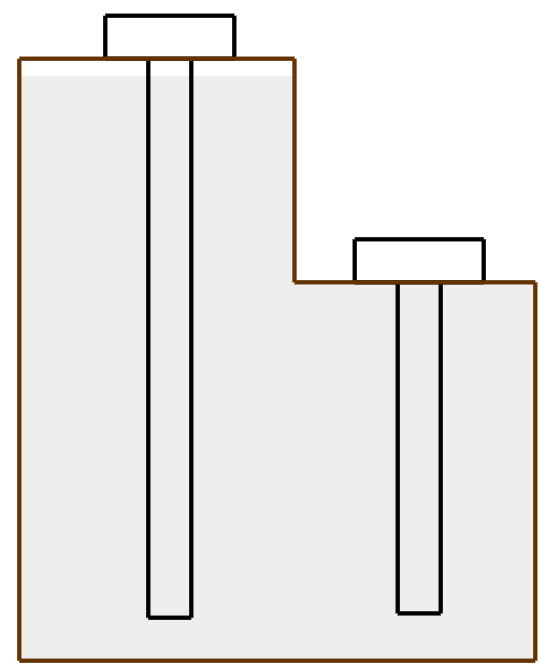
\includegraphics[width=0.9\linewidth]{graphics/screenshot004}
		\end{figure}
	\end{minipage}
	\hfill
	\begin{minipage}[h]{0.59\linewidth}
		Допустим, что данный бак рассчитан на 140 литров, а максимальное показание, которое может увидеть второй (правый) ДУТ - 100 литров. Далее для него начинается слепая зона.
		\bigbreak
		Если бак полон, будут присланы значения $D_1$ и $D_2$ соответствующие 140 и 100 литрам, и тогда уровень топлива:
		$$fuel = \frac{fuel_1 + fuel_2}{2} = 120$$	
	\end{minipage}
\end{frame}

\begin{frame}{Цель и задачи}
	Цель: улучшение точности измерения количества топлива в баках сложной конфигурации при использовании нескольких датчиков уровня топлива.
	\bigbreak 
	Задачи:
	\begin{enumerate}
		\item исследовать существующие подходы к решению задач определения уровня топлива в баках сложной конфигурации.
		\item определить требования к программному обеспечению.
		\item разработать и реализовать в программном обеспечении алгоритм адаптации данных, получаемых с датчиков уровня топлива для систем спутникового мониторинга.
		\item провести тестирование разработанного продукта.
		\item описать алгоритм для специалистов технической поддержки по внедрению метода вычислений в системы спутникового мониторинга.			
	\end{enumerate}
\end{frame}	

\begin{frame}{Решение}
	Рассмотрим бак следующей конфигурации с тремя датчиками:
	\begin{figure}
		\centering
		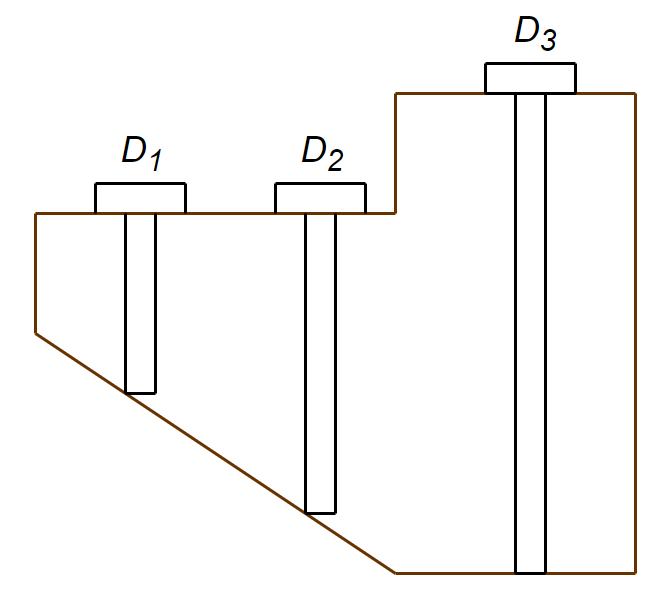
\includegraphics[width=0.6\linewidth]{graphics/screenshot005}
	\end{figure}
\end{frame}	

\begin{frame}{Этап 1: выделение зон}
	В баке выделяются зоны на основании множества ДУТов, покрывающих данный уровень:
	\\
	\begin{minipage}[h]{0.45\linewidth}
		\begin{figure}
				\centering
				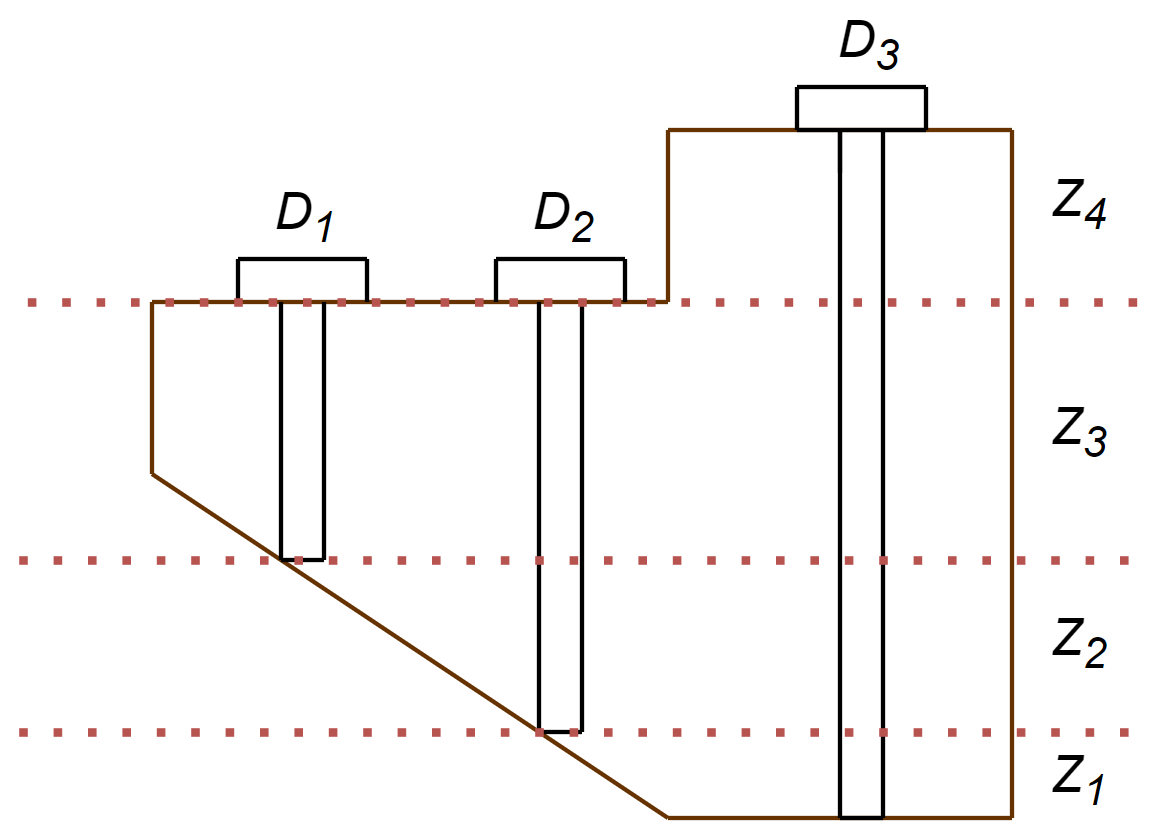
\includegraphics[width=1\linewidth]{graphics/screenshot006}
		\end{figure}
	\end{minipage}
	\hfill
	\begin{minipage}[h]{0.5\linewidth}
		$$fuel(Z_1) = f_3(D_3)$$
		$$fuel(Z_2) = \frac{f_2 (D_2)+f_3 (D_3)}{2}$$
		$$fuel(Z_3) = \frac{f_1 (D_1)+f_2(D_2)+f_3(D_3))}{3}$$
		$$fuel(Z_4)=  f_3 (D_3 )$$
	\end{minipage}
	\bigbreak
	В данном виде значение не может быть рассчитано:
	\begin{itemize}
		\item Формула имеет разветвляющуюся структуру;
		\item Для вычисления зоны надо знать уровень топлива, но чтобы знать уровень топлива - надо знать зону.
	\end{itemize}
\end{frame}

\begin{frame}{Этап 2: получение виртуальных датчиков}
	Назовём виртуальным датчиком уровня топлива (ВДУТ) некоторый отрезок ДУТа. Границы зон $Z_1,..., Z_4$ разделяют физические датчики $D_1,...,D_3$ на множество виртуальных $V_1,...,V_7$: 
	\\
	\begin{figure}
		\centering
		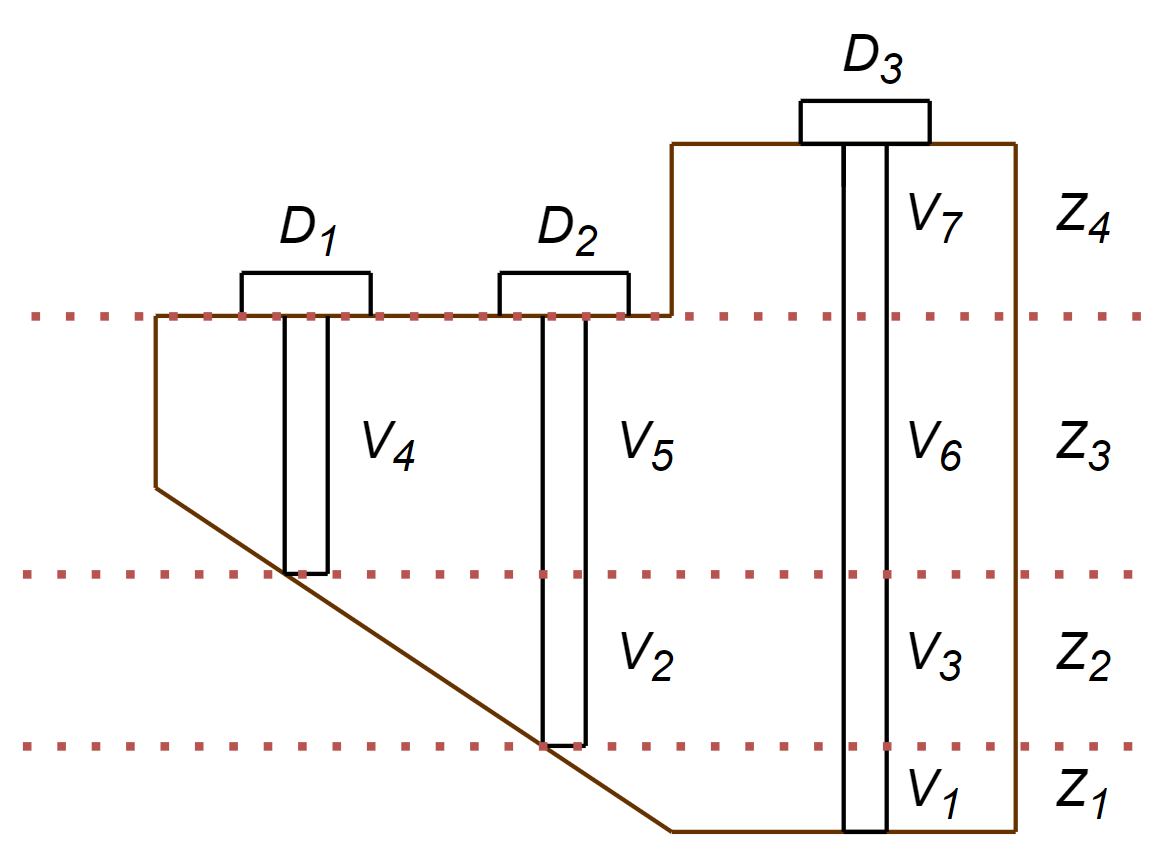
\includegraphics[width=0.45\linewidth]{graphics/screenshot008}
	\end{figure}
	Важно помнить, что датчик задаётся множеством точек~$\{(D_i,\; V_i)\}$. Каждому из виртуальных датчиков необходимо сопоставить множество точек на ДУТе.
\end{frame}

\begin{frame}{Этап 3: получение тарировок ВДУТ}
	Процесс разбиения $D_3$ на виртуальные датчики:
	\begin{figure}
	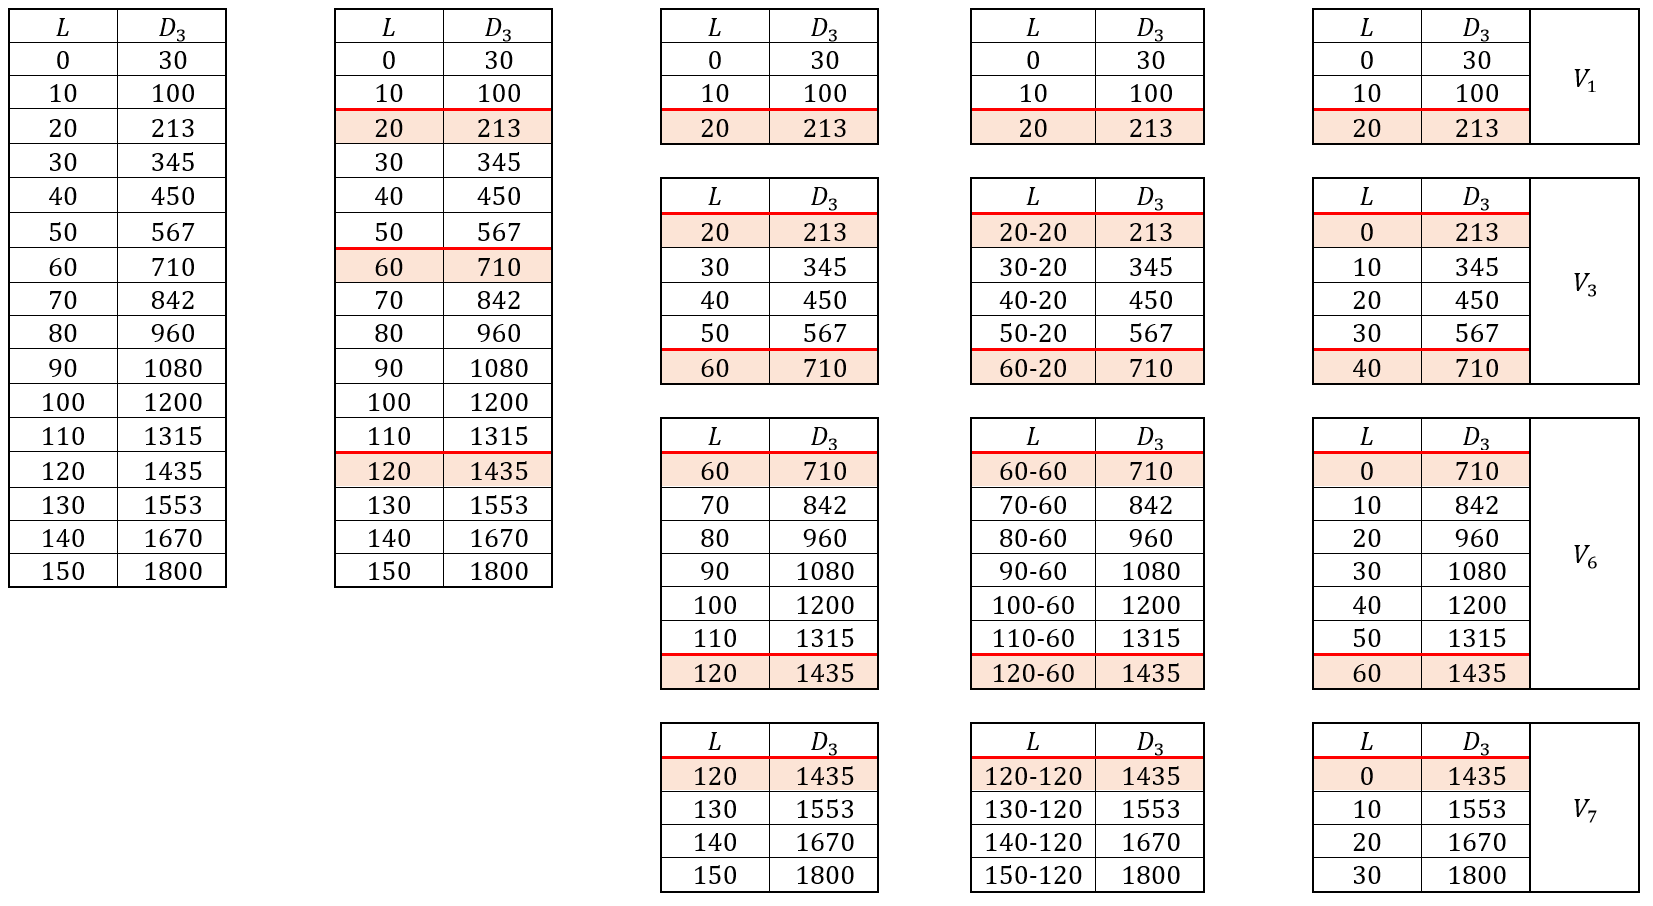
\includegraphics[width=1.05\linewidth]{graphics/screenshot007}
	\end{figure}
\end{frame}

\begin{frame}{Этап 4: подавление экстраполяции}
	Чтобы вычисления происходили корректно, необходимо подавить экстраполяцию. Достаточно добавить две точки, которые бы дублировали показания литров, но отличались на единицу в показаниях на ДУТе:
	\begin{figure}
		\centering
		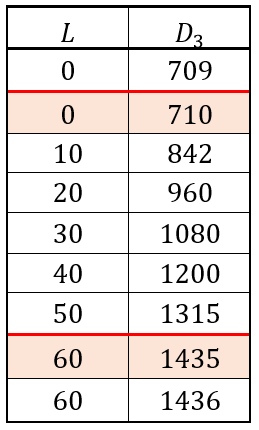
\includegraphics[width=0.2\linewidth]{graphics/screenshot009}
	\end{figure}
\end{frame}

\begin{frame}{Этап 5: получение формулы}
	
	\begin{minipage}[h]{0.55\linewidth}
	Наличие виртуальных датчиков с устраненной экстраполяцией от ССМ позволяет для случая получить формулу:
	\end{minipage}
	\hfill
	\begin{minipage}[h]{0.4\linewidth}
		\begin{figure}
				\centering
				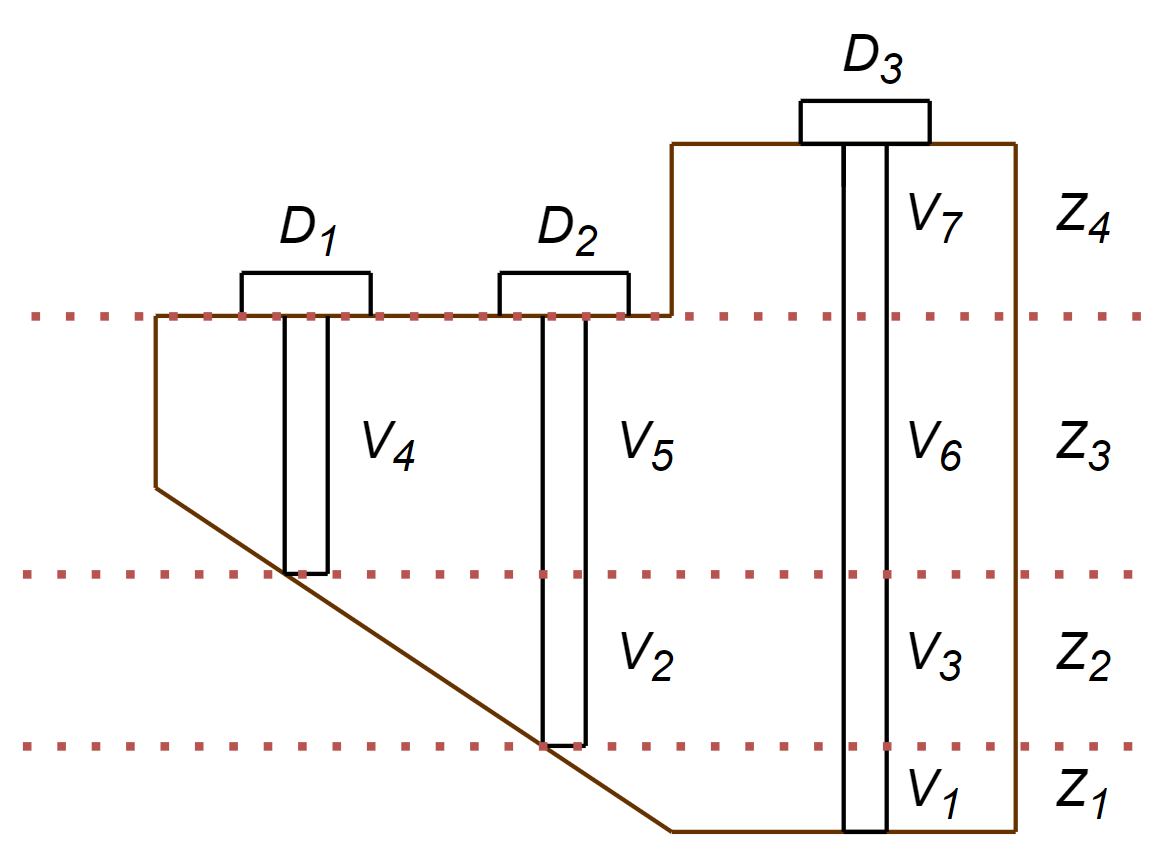
\includegraphics[width=1\linewidth]{graphics/screenshot008}
			\end{figure}
	\end{minipage}
	
	\begin{align*}
	    fuel &= f_{v_1}(D_3)+\frac{f_{v_2}(D_2)+f_{v_3}(D_3)}{2} +  \\        
	         &+ \frac{f_{v_4}(D_1)+f_{v_5} (D_2)+f_{v_6}(D_3)}{3}+f_{v_7}(D_3)
	\end{align*}
	где $f_{v_i}$ - функция для вычисления количества топлива для виртуального ДУТа ${v_i}$, а $D_i$ - показания с $i$-го физического датчика.
\end{frame}

\begin{frame}
	Проведенные вычисления было легко осуществить, так как мы имели представление о форме бака и местоположений датчиков.
	\bigbreak
	Была поставлена задача разработать такой продукт, который бы не имел такой информации, а ориентировался только на тарировочные таблицы.
	\bigbreak
	Более того, программа должна корректно обрабатывать баки в форме сообщающихся сосудов.
\end{frame}

\begin{frame}{Используемые инструменты}
	Язык программирования: Python 3.X
	\bigbreak
	Среда разработки: PyCharm Community
	\bigbreak
	Библиотеки:
	\begin{itemize}
		\item для чтения и записи исходных данных: xlrd, openpyxl;
		\item для обработки данных: pandas, numpy;
		\item для визуализации данных: matplotlib;
		\item для unit-тестирования: unittest.
	\end{itemize}
\end{frame}	

\begin{frame}{Результаты работы программы}
	Программа выполняет разбиение тарировочной таблицы на множество файлов:
	\begin{figure}
		\centering
		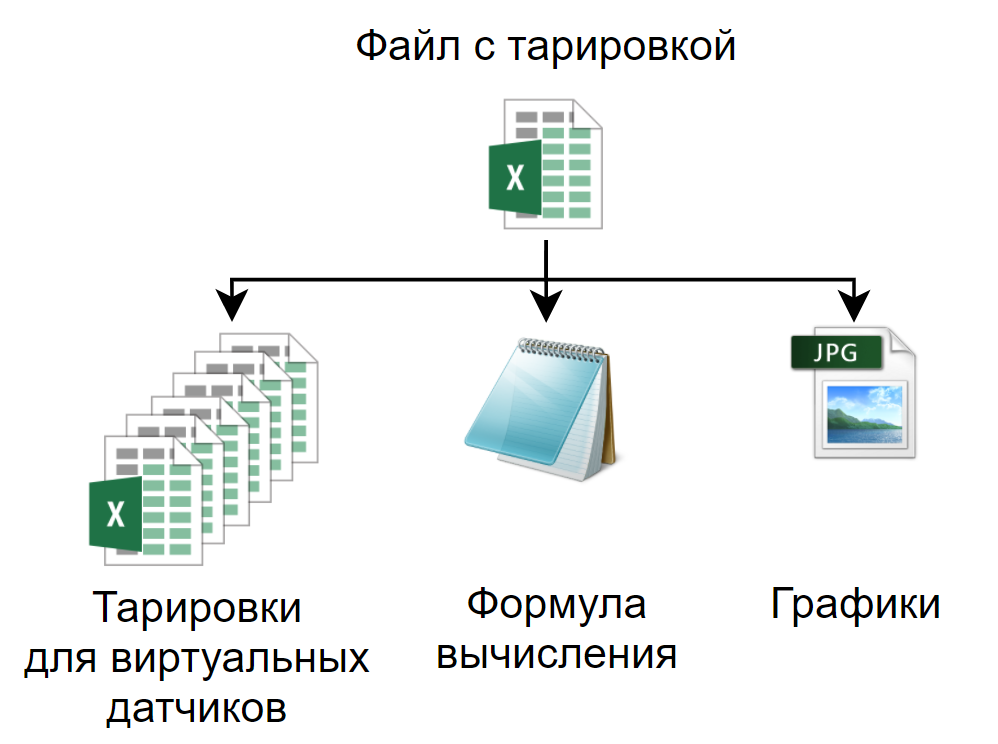
\includegraphics[width=0.7\linewidth]{graphics/screenshot010}
	\end{figure}
\end{frame}

\begin{frame}
	\begin{figure}
	\centering
	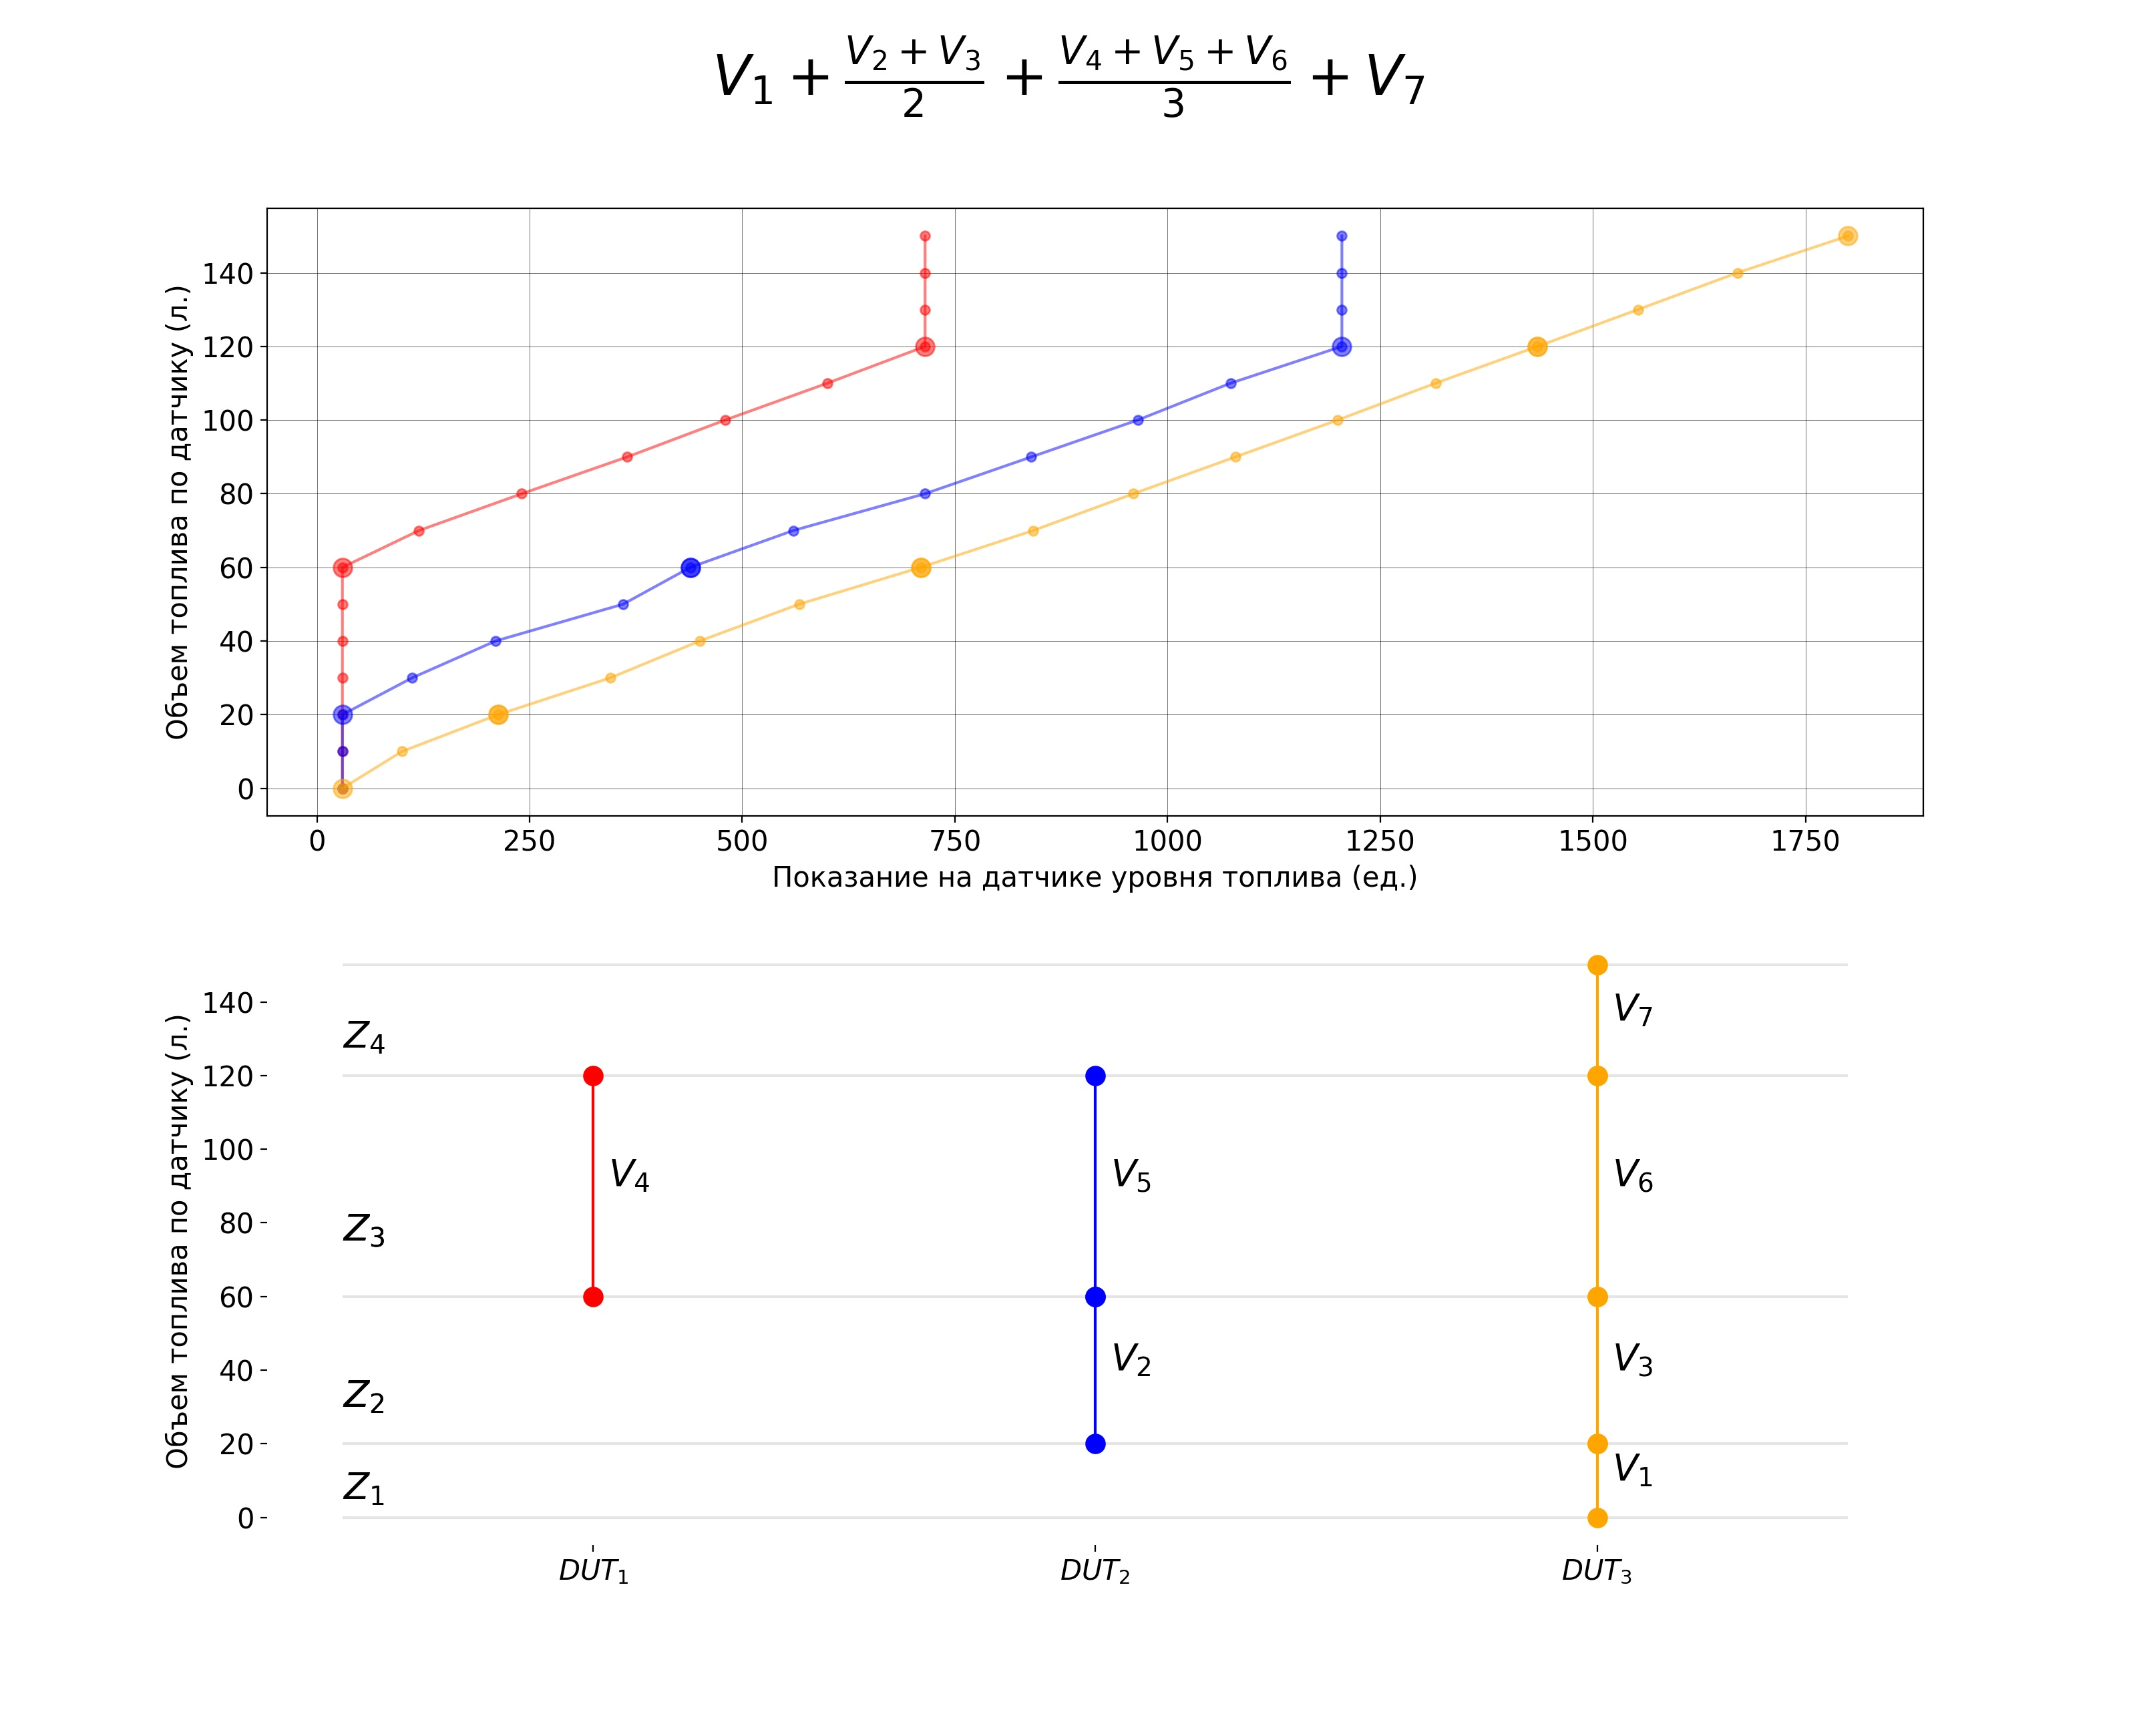
\includegraphics[width=0.95\linewidth]{../Программа/test/test_main/tmp2/plot}
	\end{figure}
\end{frame}

\begin{frame}
	\begin{figure}
	\centering
	\includegraphics[width=1.05\linewidth]{C:/Users/John/Desktop/MAN/plot}
	\end{figure}
\end{frame}

\begin{frame}
	\begin{figure}
	\centering
	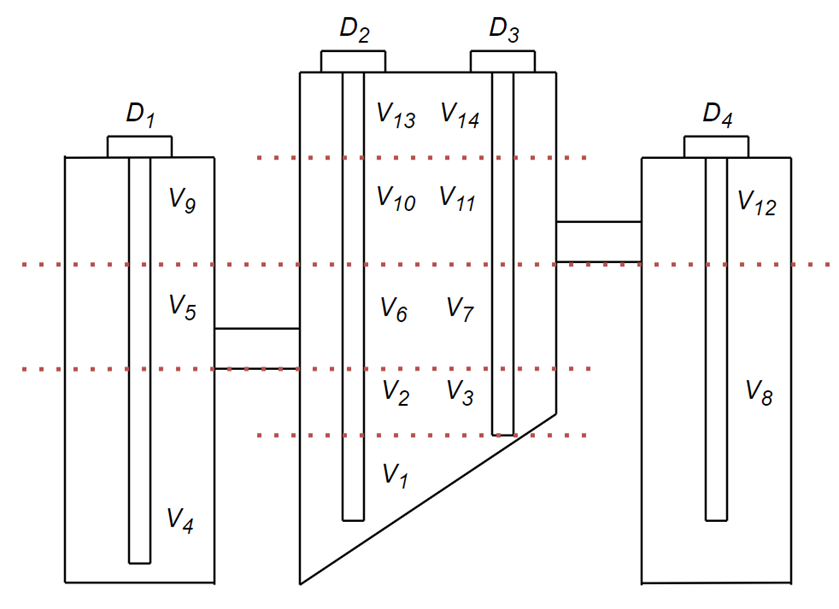
\includegraphics[width=0.85\linewidth]{graphics/screenshot011}
	Конфигурация бака для слайда №20
	\end{figure}
\end{frame}

\begin{frame}
	\begin{figure}
	\centering
	\includegraphics[width=1.05\linewidth]{C:/Users/John/Desktop/test1/plot}
	\end{figure}
\end{frame}

\begin{frame}{Структура проекта. Тестирование}
	
	\begin{minipage}[h]{0.39\linewidth}
		\begin{figure}
			\centering
			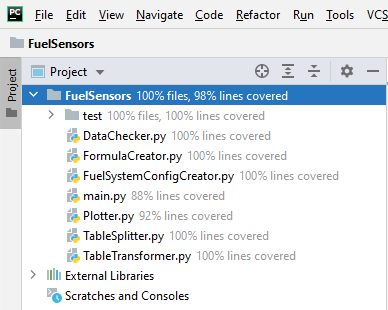
\includegraphics[width=1\linewidth]{graphics/screenshot001}
		\end{figure}
	\end{minipage}
	\hfill
	\begin{minipage}[h]{0.59\linewidth}
		\begin{itemize}
			\item Unit-тестирование. Достигнуто 98\%-е покрытие строк
			\item Инсталляционное тестирование в лаборатории технической защиты информации
			\item Эксплуатационное приёмочное тестирование в ООО "Экспертком"
		\end{itemize}
	\end{minipage}
	
\end{frame}	

\begin{frame}{Заключение}
	В рамках выпускной квалификационной работы:
	\begin{enumerate}
		\item исследованы подходы повышения точности вычисления уровня топлива;
		\item разработан и реализован алгоритм на ЯП Python для разбиения тарировочной таблицы на виртуальные датчики уровня топлива, получения формулы вычисления и построения графиков;
		\item проведено unit-тестирование, инсталляционное, эксплуатационное приёмочное тестирования;
		\item описан алгоритм действия для специалистов технической поддержки по внедрению метода вычислений на примере ССМ wialon.			
	\end{enumerate}
\end{frame}	

\end{document}
